\documentclass{standalone}
\usepackage{xcolor}
\usepackage{verbatim}
\usepackage[T1]{fontenc}
\usepackage{graphics}
\usepackage{hyperref}
\newcommand{\code}[1]{\texttt{#1}}
\newcommand{\R}{R}
\newcommand{\pkg}[1]{#1}
\newcommand{\CRANpkg}[1]{\pkg{#1}}%
\newcommand{\BIOpkg}[1]{\pkg{#1}}
\usepackage{amsmath,amssymb,array}
\usepackage{booktabs}
\providecommand{\tightlist}{%
  \setlength{\itemsep}{0pt}\setlength{\parskip}{0pt}}
\newlength{\cslhangindent}
\setlength{\cslhangindent}{1.5em}
\newlength{\csllabelwidth}
\setlength{\csllabelwidth}{3em}
\newlength{\cslentryspacingunit} % times entry-spacing
\setlength{\cslentryspacingunit}{\parskip}
\newenvironment{cslreferences}%
  {}%
  {\par}
\newenvironment{CSLReferences}[2] % #1 hanging-ident, #2 entry spacing
 {% don't indent paragraphs
  \setlength{\parindent}{0pt}
  % turn on hanging indent if param 1 is 1
  \ifodd #1
  \let\oldpar\par
  \def\par{\hangindent=\cslhangindent\oldpar}
  \fi
  % set entry spacing
  \setlength{\parskip}{#2\cslentryspacingunit}
 }%
 {}
\usepackage{calc}
\newcommand{\CSLBlock}[1]{#1\hfill\break}
\newcommand{\CSLLeftMargin}[1]{\parbox[t]{\csllabelwidth}{#1}}
\newcommand{\CSLRightInline}[1]{\parbox[t]{\linewidth - \csllabelwidth}{#1}\break}
\newcommand{\CSLIndent}[1]{\hspace{\cslhangindent}#1}
\usepackage{subcaption}
\usepackage{tikz}
\usepackage{cleveref}
\usetikzlibrary{positioning}
\usetikzlibrary{shapes.geometric, arrows}
\DeclareMathOperator{\one}{\mathbf{1}}
\DeclareMathOperator{\Var}{var}
\def\sectionautorefname{Section}
\def\subsectionautorefname{Section}

\begin{document}
\nopagecolor
\centering
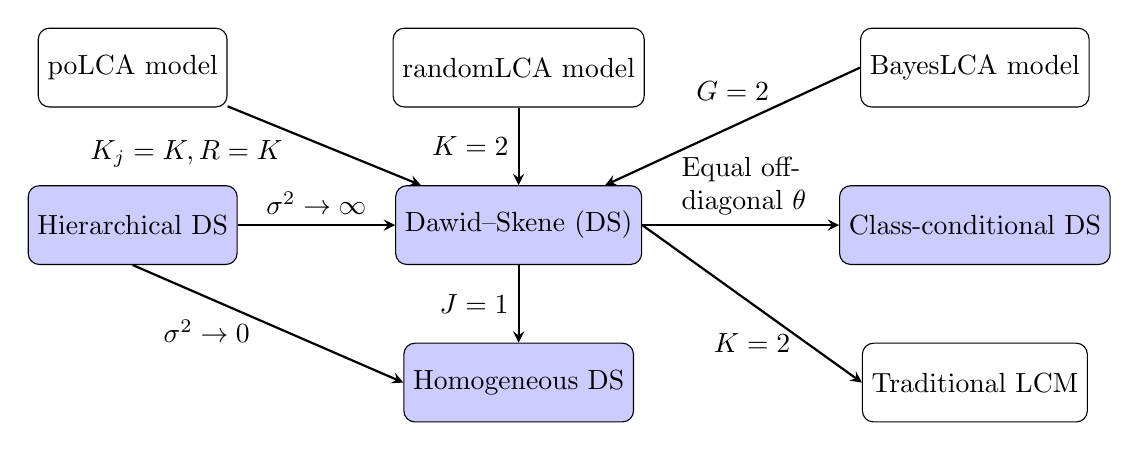
\begin{tikzpicture}[node distance=2cm]
\tikzstyle{rater}=[
    rectangle,
    rounded corners,
    minimum width=2cm,
    minimum height=1cm,
    text centered,
    fill=blue!20!white,
    draw=black
]
\tikzstyle{other}=[
    rectangle,
    rounded corners,
    minimum width=2cm,
    minimum height=1cm,
    text centered,
    draw=black
]
\tikzstyle{arrow}=[
    thick,
    ->,
    >=stealth
]
\node [rater] (DS) {Dawid--Skene (DS)};
\node [rater, below of=DS] (HODS) {Homogeneous DS};
\node [rater, left=2cm of DS] (HIDS) {Hierarchical DS};
\node [other, above of=HIDS] (poLCA) {\CRANpkg{poLCA} model};
\node [other, above of=DS] (randomLCA) {\CRANpkg{randomLCA} model};
\node [rater, right=2.5cm of DS] (CCDS) {Class-conditional DS};
\node [other, above of=CCDS] (BayesLCA) {\CRANpkg{BayesLCA} model};
\node [other, below of=CCDS] (LCM) {Traditional LCM};
\draw [arrow] (DS) -- node[anchor=east] {$J = 1$} (HODS);
\draw [arrow] (randomLCA) -- node[anchor=east] {$K = 2$} (DS);
\draw [arrow] (BayesLCA.west) -- node[anchor=south, yshift = 0.2cm] {$G = 2$} (DS);
\draw [arrow] (poLCA) -- node[anchor=east, xshift = -0.4cm, yshift = -0.1cm] {$K_j = K, R = K$} (DS);
\draw [arrow] (HIDS) -- node[anchor=south] {$\sigma^2 \rightarrow \infty$} (DS);
\draw [arrow] (HIDS.south) -- node[xshift = -0.1cm, yshift = -0.1cm, anchor=east] {$\sigma^2 \rightarrow 0$} (HODS.west);
\draw [arrow] (DS) -- node[text width=2.1cm, xshift = 0.3cm, yshift = -0.2, anchor=south] {Equal off-diagonal $\theta$} (CCDS);
\draw [arrow] (DS.east) -- node[yshift = -0.5cm] {$K = 2$} (LCM.west);
\end{tikzpicture}
\end{document}
